\problemname{\problemyamlname}

\illustration{0.3}{musicalchairs.jpg}{
  A family playing Musical Chairs. \\
  CC BY-SA 3.0 by Artaxerxes on \href{https://commons.wikimedia.org/wiki/File:Musical_chairs_Lawn_Jam_Our_Community_Place_Harrisonburg_VA_June_2008.jpg}{Wikimedia Commons}
}%
In a deterministic version of \emph{Musical Chairs}\footnote{You do not need to know the original game, but you can try to play it after the contest is over.}, there are $n$ chairs placed in a circle.
The chairs are numbered from~$1$ to~$n$ in clockwise order.
Initially, the~$i$th player sits on the~$i$th chair.
During the game, the game master gives commands to all players at once.

The first type of command tells each player to move~$x$ chairs farther in clockwise order,
so they must move from chair~$i$ to chair~$i+x$.

The second type of command tells each player to move from chair~$i$ to chair~$i\cdot{}x$.
Both these calculations are done modulo $n$, where a remainder of $0$ corresponds to chair $n$.

If two or more people want to move to the same chair,
then the player needing to travel the least in clockwise direction to reach the chair gets to take the seat,
and the other players trying to reach the same chair are out of the game.
This is illustrated in Figure~\ref{fig:chairs},
where the larger circles represent the chairs and their numbers are written on their inside.
The smaller circles represent the players.
The next command (\texttt{* 10}) tells player~$10$ (now on seat~$11$) and player~$4$ (now on seat~$5$) to move to chair~$2$.
However, since player~$10$ needs to travel less, this player gets to take the seat.
Note that the other $10$ players will also move to some other chairs,
but this is omitted from the figure for the sake of readability.

\begin{figure}[!h]
  \centering
  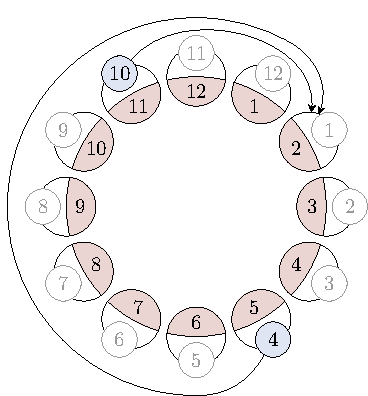
\includegraphics[width=0.45\textwidth]{sample}
  \caption{
    Illustration of Sample Input 1 at the fourth command, where players~$4$~and~$10$ need to move to chair~$2$.
    Because player~$10$ needs to travel less in clockwise direction, this player gets to take the seat.
  }
  \label{fig:chairs}
\end{figure}

The jury wasted most of their free time designing this game and now need to go back to work.
Fortunately, the game is deterministic, so you can play the game without the help of the jury.

\begin{Input}
The input consists of:
\begin{itemize}
  \item
  One line with two integers $n$ and $q$ ($2\leq n,q\leq5\cdot10^5$), the number of chairs and the number of commands.
  \item
  $q$ lines, each containing one of three command types:
  \begin{itemize}[topsep=0pt, itemsep=-2pt]
  \item ``\texttt{+~$x$}'': The player on chair~$i$ moves to chair~$i+x$.
  \item ``\texttt{*~$x$}'': The player on chair~$i$ moves to chair~$i\cdot{}x$.
  \item ``\texttt{?~$x$}'': Tell us the number of the player on chair~$x$.
  \end{itemize}
  All of the values $x$ will satisfy $1 \leq x \leq n$.
  \end{itemize}
\end{Input}
\begin{Output}
  For each command of type `\texttt{?}', output the number of the player on the requested chair.
  If the chair is currently empty, output $-1$ instead.
\end{Output}
